\section{Experimental Evaluation}\label{sec:experiments}

We evaluate PaperOEGM across four research questions: deterministic fault detection (\textbf{RQ1}), multi-harness packaging and context economics (\textbf{RQ2}), verification scalability and paranoid TeX containment (\textbf{RQ3}), and live hybrid semantic critique (\textbf{RQ4}). RQ1--RQ3 execute locally on CPU without external LLM API keys (Python 3.12.8, TeX Live 2026, \texttt{pandoc}, \texttt{pdfinfo}, Claude Code CLI 2.1.328); RQ4 runs the deterministic baseline on CPU and dispatches 15 live read-only critics on Antigravity (Gemini 4). All runs execute against an unmodified plugin codebase (\texttt{git\ diff} outside \texttt{paper\_\allowbreak{}workspace/} is empty; resolution-phase workspace updates carry recorded \texttt{git\_\allowbreak{}dirty} attestations) and write strictly non-synthetic outputs (\texttt{is\_\allowbreak{}synthetic:\ false}) registered in \texttt{experiments/\allowbreak{}provenance\_\allowbreak{}index.\allowbreak{}json}, keeping smoke checks segregated in \texttt{dry\_\allowbreak{}run/}.

\subsection{RQ1: Fault Detection and Deterministic Boundaries}\label{sec:exp-rq1}

\textbf{Setup.} We construct \textbf{PO-FaultBench}, an author-constructed corpus of 120 realistic workspaces/seed over five seeds (\texttt{42}--\texttt{46}, plus 20 adversarial evasion cases/seed = 700 live CLI evaluations). Eight positive fault families (10 cases/family, 80 positives/seed) span both \emph{schema-independent} faults (\textbf{FF1a}, \textbf{FF5}--\textbf{FF7}) and \emph{PaperOEGM-schema} checks (\textbf{FF1b}, \textbf{FF2}--\textbf{FF4}, \textbf{FF8}): \textbf{FF1} hallucinated citation missing from \texttt{.bib} (\textbf{FF1a}, 50\%) or \texttt{citation\_\allowbreak{}ledger.\allowbreak{}json} (\textbf{FF1b}, 50\%); \textbf{FF2} \texttt{unverified\_\allowbreak{}needs\_\allowbreak{}human\_\allowbreak{}check} or missing \texttt{literature/\allowbreak{}sources/} snapshot; \textbf{FF3} isolated \texttt{dry\_\allowbreak{}run/} reference, \texttt{is\_\allowbreak{}synthetic:\ true}, or unattested \texttt{user\_\allowbreak{}byo}; \textbf{FF4} decimal drift beyond \(\epsilon(d)\) under inline \texttt{run:\textless{}id\textgreater{}} or unregistered \texttt{run\_\allowbreak{}id}; \textbf{FF5} \texttt{.md}-to-\texttt{.tex} dropped citation, \texttt{\textbackslash{}label\{\}}, or decimal; \textbf{FF6} double-blind path, GitHub URL (incl.~\texttt{\%} comments), \texttt{\textbackslash{}iclrfinalcopy}, or \texttt{\textbackslash{}usepackage\{cvpr\}}; \textbf{FF7} Zip Slip (\texttt{../}), symlink, or active \texttt{\textbackslash{}write18} in \texttt{.zip}/\allowbreak{}\texttt{.tar.\allowbreak{}gz} templates; and \textbf{FF8} \texttt{check-readonly} mutation or \texttt{state-sync} digest drift.

Forty hard negative controls/seed test valid rounding and \(0\text{--}1 \to \%\) conversion, attested \texttt{user\_\allowbreak{}provided}/\allowbreak{}\texttt{user\_\allowbreak{}byo} runs, LaTeX dimensions (\texttt{0.92\textbackslash{}linewidth}, \texttt{10.5pt}) with commented \texttt{\%\ \textbackslash{}write18}, camera-ready URLs/flags, and clean snapshots. Twenty \textbf{Adversarial Evasion} cases/seed inject non-syntactic attacks: integer-only count falsification (\textbf{E1}), macro-obfuscated \texttt{\textbackslash{}csname\ write18\textbackslash{}endcsname} (\textbf{E2}), valid-key semantic citation distortion (\textbf{E3}), and prose lab deanonymization without paths/URLs (\textbf{E4}). We compare \textbf{PaperOEGM Full} (live \texttt{po\_\allowbreak{}tools.\allowbreak{}py}), \textbf{B1 (No Inline Provenance)} filtering inline decimal blockers from \texttt{po\_\allowbreak{}tools.\allowbreak{}py} output (latency omitted as ---), and \textbf{B0 (Compiler-Only)} scored analytically for standard \texttt{pdflatex}/\allowbreak{}\texttt{bibtex} missing-key/file errors (latency ---).

\begin{table*}[t]
\centering
\footnotesize
\setlength{\tabcolsep}{4pt}
\caption{PO-FaultBench detection across $n=5$ seeds (80 positive faults, 40 hard negative controls, and 20 adversarial evasions/seed; mean $\pm$ SD). B0/B1 latencies are omitted (---) as analytical/filtered baselines.}
\label{tab:faultbench}
\begin{tabular}{lcccccc}
\toprule
\textbf{System / Condition} & \textbf{Recall (\%)} & \textbf{Precision (\%)} & \textbf{F1-Score (\%)} & \textbf{FPR (\%)} & \textbf{Evasion Recall (\%)} & \textbf{Latency (ms)} \\
\midrule
B0: Compiler-Only & 6.25 $\pm$ 0.00 & 100.00 $\pm$ 0.00 & 11.76 $\pm$ 0.00 & 0.00 $\pm$ 0.00 & 0.00 $\pm$ 0.00 & --- \\
B1: No Inline Provenance & 87.50 $\pm$ 0.00 & 100.00 $\pm$ 0.00 & 93.33 $\pm$ 0.00 & 0.00 $\pm$ 0.00 & 0.00 $\pm$ 0.00 & --- \\
\textbf{PaperOEGM Full (\texttt{po\_\allowbreak{}tools.\allowbreak{}py})} & \textbf{100.00 $\pm$ 0.00} & \textbf{100.00 $\pm$ 0.00} & \textbf{100.00 $\pm$ 0.00} & \textbf{0.00 $\pm$ 0.00} & \textbf{0.00 $\pm$ 0.00} & \textbf{108.20 $\pm$ 2.07} \\
\bottomrule
\end{tabular}
\end{table*}

\textbf{Results.} Table~\ref{tab:faultbench} and Figure~\ref{fig:faultbench} show PaperOEGM Full achieving 100.0\% recall, 100.0\% precision, 100.0\% F1-score, and 0.0\% FPR in 108.20 \(\pm\) 2.07 ms/workspace. Compiler-Only (B0) reaches 6.25\% recall (catching only the 50.0\% FF1a missing-\texttt{.bib} subset while missing FF1b and FF2--FF8), and disabling inline \texttt{run:\textless{}id\textgreater{}} auditing (B1) drops recall to 87.5\% (93.33\% F1-score) by missing 100.0\% of FF4.

Below the dashed divider in Figure~\ref{fig:faultbench}, all three deterministic systems record \textbf{0.0\% recall} across E1--E4. Because \texttt{po\_\allowbreak{}tools.\allowbreak{}py} and PO-FaultBench were co-authored, main-suite recall verifies specification compliance rather than security completeness; the 0.0\% evasion boundary empirically motivates native TeX containment (RQ3) and fresh semantic critics (RQ4).

\begin{figure*}[t]
\centering
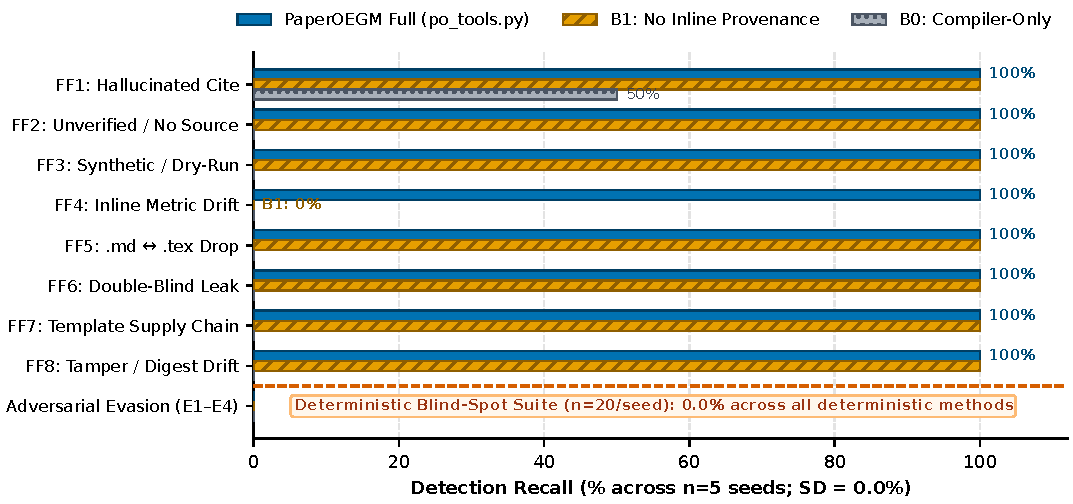
\includegraphics[width=0.88\textwidth]{figures/fig_faultbench_recall.pdf}
\caption{Per-family recall (\%) on PO-FaultBench (FF1--FF8, 80 positives + 40 negative controls/seed, $n=5$, SD $= 0.0\%$) and 20-case/seed adversarial evasion suite across PaperOEGM Full, B1 (No Inline Provenance), and B0 (Compiler-Only).}
\label{fig:faultbench}
\end{figure*}

\subsection{RQ2: Packaging, Context Footprint, and Determinism}\label{sec:exp-rq2}

\textbf{Setup.} Across five build runs (\texttt{42}--\texttt{46}), we compare PaperOEGM against \textbf{B2 (Monolithic Single-Skill)} concatenating all 10 skills, \texttt{execution\_\allowbreak{}instructions.\allowbreak{}md}, 6 protocols, and 5 review standards, and \textbf{B3 (Public EGM Reference)} measured on open-source \texttt{google/\allowbreak{}elephant-goldfish-model} v0.1.1 \citep{google2026egm} (scoped strictly to skill/agent footprint; non-applicable cells marked ---). We report whole-file \texttt{SKILL.\allowbreak{}md} bytes (decimal KB = 1,000 B for loader ceilings; binary KiB = 1,024 B for ZIP archives), active-stage load, startup frontmatter size, compliance defects \citep{zhang2026reusable}, live \texttt{claude\ plugin\ validate}, and deterministic ZIP SHA-256 parity across \texttt{antigravity}, \texttt{claude}, and \texttt{openai} via \texttt{scripts/\allowbreak{}pack\_\allowbreak{}plugin.\allowbreak{}py}.

\begin{table*}[t]
\centering
\footnotesize
\setlength{\tabcolsep}{4pt}
\caption{Multi-harness skill footprint, context reduction, compliance defects, and deterministic build parity ($n=5$ builds). Non-applicable baseline cells are marked ---; public EGM (B3) is scoped strictly to skill/agent footprint.}
\label{tab:packaging}
\begin{tabular}{lccccccc}
\toprule
\textbf{Packaging Strategy} & \textbf{Skills} & \textbf{Median / Max Skill (B)} & \textbf{Active Stage (B)} & \textbf{vs. Mono (\%)} & \textbf{Max Agent (B)} & \textbf{Defects} & \textbf{ZIP SHA-256} \\
\midrule
B2: Monolithic Single-Skill & 1 & 79,454 / 79,454 & 79,454 & 0.00\% & --- & --- & --- \\
B3: Public EGM Reference & 7 & 15,205 / 24,257 & --- & --- & 7,355 & --- & --- \\
\textbf{PaperOEGM (10 Skills)} & \textbf{10} & \textbf{3,900 / 4,526} & \textbf{14,171} & \textbf{-82.16\%} & \textbf{2,376} & \textbf{0} & \textbf{100.0\%} \\
\bottomrule
\end{tabular}
\end{table*}

\textbf{Results.} In Table~\ref{tab:packaging} and Figure~\ref{fig:footprint}, every PaperOEGM \texttt{SKILL.\allowbreak{}md} spans 3,466--4,526 bytes (median 3,900 B, maximum 63 lines)---preserving 62.28\% headroom below our 12 KB budget and 81.14\% below Antigravity's 24 KB (24,000 B) ceiling, whereas public EGM (B3) reaches 15,205 B median and 24,257 B max (+257 B over the 24,000 B limit; max agent 7,355 vs.~2,376 B). Protocol offloading reduces median active-stage context from 79,454 B (B2) to 14,171 B (-82.16\%; 15,749 B max stage) and startup index context to 2,270 B (-97.14\%). PaperOEGM yields 0 compliance defects, passes \texttt{claude\ plugin\ validate} cleanly, and produces byte-identical ZIPs (124.88 KiB Antigravity, 142.37 KiB Claude, 125.75 KiB OpenAI; 100.0\% SHA-256 parity) in 143.00 \(\pm\) 10.09 ms.

\begin{figure*}[t]
\centering
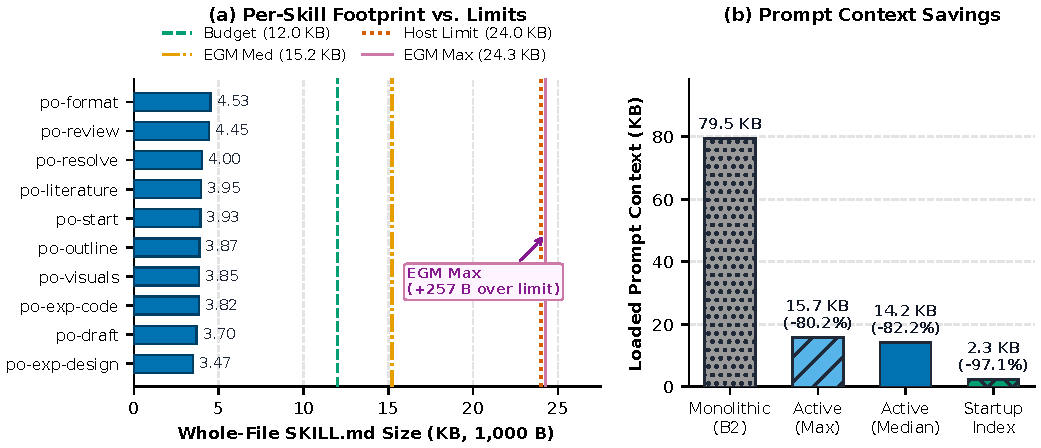
\includegraphics[width=0.88\textwidth]{figures/fig_skill_footprint.pdf}
\caption{Skill packaging footprint and context economics: (a) whole-file \texttt{SKILL.\allowbreak{}md} size (decimal KB, 1,000 B) across 10 PaperOEGM skills vs. 12 KB budget, public EGM v0.1.1 median/max (+257 B over ceiling), and Antigravity's 24 KB ceiling; (b) loaded prompt context across Monolithic (B2), active max/median, and startup index.}
\label{fig:footprint}
\end{figure*}

\subsection{RQ3: Scalability, Offloading, and Paranoid TeX Containment}\label{sec:exp-rq3}

\textbf{Setup.} We benchmark live subprocess runs of all four \texttt{po\_\allowbreak{}tools.\allowbreak{}py} subcommands across four scales over \(n=5\) seeds: \textbf{S} (20 cites, 5 runs), \textbf{M} (50/10), \textbf{L} (80/20), and \textbf{XL} (120/30), against a pre-experiment \texttt{\textless{}\ 250\ ms} XL target and \texttt{\textgreater{}\ 2,\allowbreak{}000\ ms} falsification bar. Each seed also runs two paranoid TeX suites (\texttt{openin\_\allowbreak{}any=p\ openout\_\allowbreak{}any=p\ pdflatex\ \mbox{-{}-}no-\allowbreak{}shell-escape}): (1) double-blind builds across \textbf{ACM SIGPLAN} (\texttt{acmart{[}sigplan,\allowbreak{}review,\allowbreak{}anonymous{]}}), \textbf{CVPR 2025}, and \textbf{ICLR 2025} audited via \texttt{pdfinfo} and \texttt{format-verify}; and (2) a \textbf{3-vector adversarial suite} executing E2 \texttt{\textbackslash{}csname\ write18\textbackslash{}endcsname}, parent \texttt{\textbackslash{}openout\ ../\allowbreak{}pwn\_\allowbreak{}out.\allowbreak{}txt}, and parent \texttt{\textbackslash{}openin\ ../\allowbreak{}secret\_\allowbreak{}parent.\allowbreak{}txt} (checked via \texttt{pdftotext}).

\textbf{Results.} Figure~\ref{fig:scalability}(a) shows 4-command latency staying flat from 266.00 \(\pm\) 7.28 ms (S) to 268.55 \(\pm\) 6.80 ms (XL; M: 265.49 \(\pm\) 4.94 ms, L: 262.39 \(\pm\) 7.84 ms; XL breakdown: \texttt{state-sync} 125.52 \(\pm\) 2.81, \texttt{check-readonly} 58.07 \(\pm\) 3.56, \texttt{review-preflight} 43.06 \(\pm\) 3.75, \texttt{format-verify} 41.91 \(\pm\) 3.51 ms). Figure~\ref{fig:scalability}(b) shows \texttt{literature/\allowbreak{}sources/} offloading saves 87.82\% (S) to 87.96\% (XL; 24,169 B loaded vs.~176,550 B offloaded). All 3/3 double-blind venues compile (\texttt{acmart{[}sigplan{]}} 1698.11 \(\pm\) 27.14 ms, \texttt{cvpr2025} 1285.42 \(\pm\) 28.64 ms, \texttt{iclr2025} 982.74 \(\pm\) 7.24 ms) with 0 identity leaks. On the adversarial suite, paranoid \texttt{pdflatex} blocks \textbf{2/3} exploits across all five seeds: E2 \texttt{\textbackslash{}csname\ write18\textbackslash{}endcsname} (1.0) and parent \texttt{\textbackslash{}openout} (1.0) are blocked, whereas parent \texttt{\textbackslash{}openin} read traversal is \textbf{not blocked} (0.0).

Three practical findings follow. First, XL latency (268.55 ms) slightly exceeded our 250 ms target (still \textgreater7\(\times\) below 2,000 ms) due to fixed cold Python startup across four processes; marginal 6\(\times\) scale growth is only +2.55 ms. Second, \texttt{cvpr2025}/\allowbreak{}\texttt{iclr2025} blank all three PDF identity fields, whereas \texttt{acmart} v2.16 injects a generic non-identifying \texttt{Creator:\ LaTeX\ with\ acmart\ ...} string via \texttt{hyperxmp} (1 generic tag, 0 identity leaks). Third, inspecting TeX Live 2026's \texttt{texmf.\allowbreak{}cnf} confirmed upstream TeX Live 2026 retired \texttt{openin\_\allowbreak{}any} into a silent no-op (always permitting input reads even when \texttt{kpsewhich} echoes \texttt{p}), proving untrusted templates require OS-level sandboxing (containers or \texttt{sandbox-exec}) alongside \texttt{\mbox{-{}-}no-\allowbreak{}shell-escape} and \texttt{openout\_\allowbreak{}any=p}.

\begin{figure*}[t]
\centering
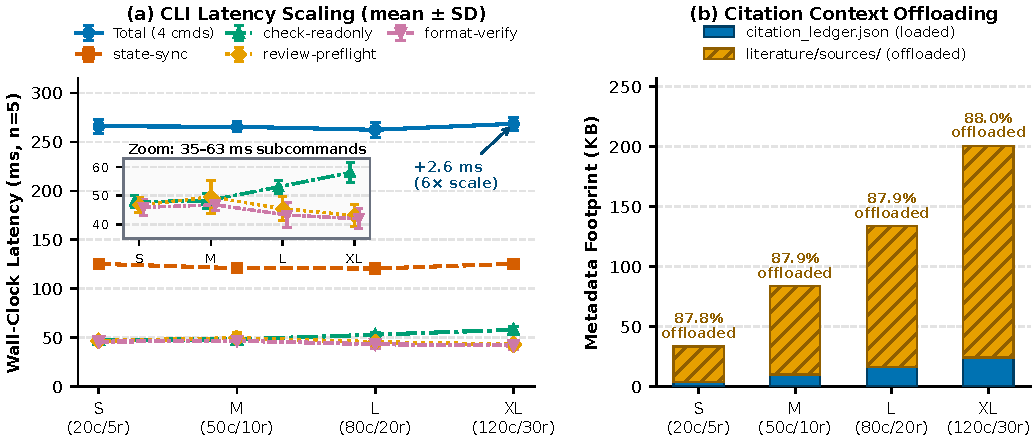
\includegraphics[width=0.88\textwidth]{figures/fig_scalability.pdf}
\caption{Verification scalability across S (20c/5r) to XL (120c/30r), $n=5$: (a) wall-clock CLI latency (mean $\pm$ SD) with 35--63 ms zoomed inset; (b) compact \texttt{citation\_\allowbreak{}ledger.\allowbreak{}json} vs. offloaded \texttt{literature/\allowbreak{}sources/} footprint (\% of total citation metadata offloaded).}
\label{fig:scalability}
\end{figure*}

\subsection{RQ4: Live Hybrid Fresh-Context Critic Audit}\label{sec:exp-rq4}

\textbf{Setup.} We construct \(n=3\) compact seeded mini-paper workspaces (\textasciitilde150--180 words across two sections each) spanning ML Systems (\texttt{s42}), Vision Benchmarks (\texttt{s43}), and Agent Security (\texttt{s44}). Each embeds 10 ground-truth defects stored outside the workspace: 5 mechanical (\textbf{M1} missing citation, \textbf{M2} unverified citation, \textbf{M3} decimal drift, \textbf{M4} synthetic/\texttt{dry\_\allowbreak{}run} leak, \textbf{M5} double-blind path/URL leak) and 5 semantic/evasion (\textbf{S1} \texttt{verified\_\allowbreak{}source} claim-vs-abstract distortion, \textbf{S2} integer-only count falsification, \textbf{S3} omitted ablation + overclaim + prose lab deanonymization, \textbf{S4} undefined math symbol + acronym, \textbf{S5} real \texttt{matplotlib} PNG rendered with colliding x-ticks, 4.5pt labels, missing units, and red-green bars). We run timed \texttt{po\_\allowbreak{}tools.\allowbreak{}py} (\texttt{review-preflight} + \texttt{format-verify}) as \textbf{B4 (Deterministic-Only)}, verify pre/post \texttt{check-readonly}, dispatch all five live read-only \texttt{po-*} critics flat in parallel on Antigravity (Gemini 4; 15 invocations), estimate output tokens via a whitespace proxy (\(\text{round}(\text{words}\times 1.3)\)), and track \texttt{clean\_\allowbreak{}control\_\allowbreak{}fp} on whether critics falsely flag the valid citation missing/unverified or the accurate secondary decimal mismatched.

\begin{table*}[t]
\centering
\footnotesize
\setlength{\tabcolsep}{4pt}
\caption{Live hybrid audit across $n=3$ compact seeded domain manuscripts (30 planted defects: 15 mechanical M1--M5, 15 semantic S1--S5; 15 live Antigravity read-only critic invocations; token counts via whitespace word-count proxy).}
\label{tab:hybrid}
\begin{tabular}{lcccccc}
\toprule
\textbf{Review Configuration} & \textbf{Mech. Recall (\%)} & \textbf{Sem. Recall (\%)} & \textbf{Total Recall (\%)} & \textbf{Clean FP} & \textbf{Mutations} & \textbf{Max Critic Tok.} \\
\midrule
B4: Deterministic-Only (\texttt{po\_\allowbreak{}tools.\allowbreak{}py}) & 100.0 $\pm$ 0.0 & 0.0 $\pm$ 0.0 & 50.0 $\pm$ 0.0 & 0.0 $\pm$ 0.0 & 0.0 & 0 \\
Fresh Read-Only Critics Alone (5 agents) & 100.0 $\pm$ 0.0 & 100.0 $\pm$ 0.0 & 100.0 $\pm$ 0.0 & 0.0 $\pm$ 0.0 & 0.0 & 1411.0 $\pm$ 35.68 \\
\textbf{PaperOEGM Hybrid (Full)} & \textbf{100.0 $\pm$ 0.0} & \textbf{100.0 $\pm$ 0.0} & \textbf{100.0 $\pm$ 0.0} & \textbf{0.0 $\pm$ 0.0} & \textbf{0.0} & \textbf{1411.0 $\pm$ 35.68} \\
\bottomrule
\end{tabular}
\end{table*}

\textbf{Results.} Table~\ref{tab:hybrid} shows B4 catching 100.0\% of M1--M5 in 91.71 \(\pm\) 0.26 ms at zero tokens but 0.0\% of S1--S5 (50.0\% total). Live flat-parallel critics recover 100.0\% of planted semantic flaws across all three domains (including multimodal inspection of \texttt{fig\_\allowbreak{}results.\allowbreak{}png} and integer count reconciliation), lifting recall to 100.0\% with 0.0 clean-control FPs, 0.0 workspace mutations, and all 15 runs within 1,500 tokens (mean peak 1411.0 \(\pm\) 35.68; \texttt{po-clarity-reader} 1400.33 \(\pm\) 48.81, \texttt{po-peer-reviewer} 1363.0 \(\pm\) 44.19, \texttt{po-visual-format-critic} 1108.33 \(\pm\) 64.78, \texttt{po-citation-auditor} 923.33 \(\pm\) 31.79, \texttt{po-evidence-auditor} 830.67 \(\pm\) 31.34).

Two scope qualifications apply. First, because critics also caught 100.0\% of M1--M5 on these compact drafts, RQ4 demonstrates \emph{one-way semantic lift} over B4 (0.0\% \(\to\) 100.0\%) rather than two-way recall separation; \texttt{po\_\allowbreak{}tools.\allowbreak{}py}'s necessity rests on RQ1/RQ3 (zero-stochasticity sub-110 ms checks at 120-citation scale and binary archive/SHA-256 audits impossible for shell-free read-only critics). Second, \texttt{po-citation-auditor} surfaced an unplanted template imprecision---flagging \texttt{"demonstrate\ strong\ baseline\ efficiency"} as unsupported by \texttt{wang2021tent} in \texttt{s43} (Nit) and contradicting \texttt{greshake2023indirect} in \texttt{s44} (Major)---confirming snapshot-grounded critique while illustrating that targeted \texttt{clean\_\allowbreak{}control\_\allowbreak{}fp} does not measure all unplanted findings.
